\documentclass[12pt,a4paper,openright,twoside]{book}
\usepackage[utf8]{inputenc}
\usepackage{disi-thesis}
\usepackage{code-lstlistings}
\usepackage{notes}
\usepackage{shortcuts}
\usepackage{acronym}
\usepackage{placeins}

\school{\unibo}
\programme{Corso di Laurea in Ingegneria e Scienze Informatiche}
\title{Automazione del dispiegamento di un cluster Kubernetes in ambiente OpenStack}
\author{Federico Bagattoni}
\date{\today}
\subject{Virtualizzazione ed Integrazione di Sistemi}
\supervisor{Prof. Vittorio Ghini}
\cosupervisor{Dott. Stefano Cacciaguerra}
%\morecosupervisor{Dott. CoSupervisor 2}
\session{I}
\academicyear{2024-2025}

% Definition of acronyms
\acrodef{IoT}{Internet of Thing}
\acrodef{vm}[VM]{Virtual Machine}


\mainlinespacing{1.241} % line spacing in mainmatter, comment to default (1)

\begin{document}

\frontmatter\frontispiece

\begin{abstract}	
Questo elaborato descrive un progetto di automazione del dispiegamento di un cluster Kubernetes su infrastruttura OpenStack, sviluppato nel contesto del progetto Nereide dell'Istituto Nazionale di Geofisica e Vulcanologia (INGV). L'obiettivo è semplificare l'installazione di ambienti computazionali complessi attraverso script Infrastructure-as-Code (IaC), per agevolare l'uso di Virtual Data Center (VDC) da parte di utenti non esperti.

Dopo un'analisi delle tecnologie utilizzate (OpenStack, Cloud-Init e Kubernetes), viene illustrata l'implementazione pratica: il provisioning delle macchine virtuali tramite interfaccia Horizon, l'installazione automatica dei pacchetti (tra cui containerd, kubeadm, Calico) e la configurazione del cluster. Particolare attenzione è data all'integrazione automatica dei nodi worker tramite script Bash e all'installazione dell'Ingress Controller Nginx in modalità NodePort, compatibile con le restrizioni del firewall del VDC.

Il funzionamento del cluster è stato verificato con un deployment di prova basato su Nginx, che espone due servizi web accessibili tramite routing Ingress.

Infine vengono proposti anche degli sviluppi futuri per il consolidamento del progetto, tra cui: l'integrazione di sistemi di monitoraggio (es. Prometheus, Grafana), la compatibilità con altri sistemi operativi, la ridondanza dei nodi master per aumentare la resilienza e l'adozione di buone pratiche per la manutenzione del cluster.
\end{abstract}

\begin{dedication} % this is optional
Optional. Max a few lines.
\end{dedication}

%----------------------------------------------------------------------------------------
\tableofcontents   
\listoffigures     % (optional) comment if empty
%\lstlistoflistings % (optional) comment if empty
%----------------------------------------------------------------------------------------

\mainmatter

% TODO: rileggere, andare a capo, typos
\chapter{Introduzione}
\section{Contesto e obiettivi del progetto}
Nel contesto dell'evoluzione verso una Scienza Aperta, riproducibile e collaborativa promossa da iniziative come l'European Open Science Cloud (EOSC),
l'Istituto Nazionale di Geofisica e Vulcanologia (INGV) ha sviluppato la piattaforma NEREIDE (NEw REsearch Infrastructure Datacenter for EMSO),
un'infrastruttura virtualizzata avanzata al servizio della comunità scientifica.
Al centro di questa piattaforma vi è il concetto di Virtual Data Center (VDC): 
un ambiente cloud dinamico, personalizzabile e sicuro, dove data scientist o team di ricerca possono gestire in autonomia risorse computazionali virtuali come
macchine virtuali, reti e servizi, mantenendo al contempo una separazione netta dalla gestione fisica dell'infrastruttura, affidata agli amministratori di sistema (v. \Cref{sec:vdc}).

Questa visione consente di ridurre la dipendenza da fornitori cloud commerciali, offrendo ambienti flessibili e scalabili, ottimizzati per il ciclo di vita della ricerca scientifica
e facilmente integrabili con ecosistemi federati come Blue-Cloud o il Digital Twin of the Ocean.
Il progetto NEREIDE, ospitato presso la stazione INGV di Portopalo di Capo Passero, rappresenta una concreta implementazione di questa architettura,
basata su tecnologie open-source come OpenStack per la gestione dell'infrastruttura e Ceph per lo storage distribuito\cite{cacciaguerra2024vdc}.

% Introduzione alla necessità di installare servizi da zero e l'obbiettivo del progetto
Tuttavia, la gestione di un VDC, sebbene sia semplificata rispetto a quella di un data center fisico, non include nativamente strumenti gestiti per il calcolo distribuito
e l'elaborazione dei dati. Questo progetto nasce dalla necessità di installare e configurare da zero servizi come Slurm, JupyterLab e Kubernetes creando uno stack automatizzato
basato su strumenti di Infrastructure-as-Code (IaC).

L'obiettivo del progetto è dunque quello di abilitare la creazione automatica e ripetibile di ambienti di calcolo avanzati, utilizzando tecnologie come Cloud-Init,
scripting Bash e componenti Kubernetes, con un focus specifico sul contesto didattico e prototipale. 
Questa scelta consente di offrire a studenti, ricercatori e tecnologi un laboratorio digitale accessibile e immediatamente operativo, facilitando la formazione,
la sperimentazione e l'evoluzione di idee progettuali, senza i vincoli tecnici delle infrastrutture fisiche.

% Riflessione sull'uso di cluster su infrastrutture virtualizzate.
Una riflessione importante riguarda il posizionamento di cluster come Kubernetes o Slurm su infrastrutture virtualizzate anziché fisiche.
Sebbene questa scelta possa sembrare controintuitiva per chi cerca prestazioni ottimali, soprattuto in confronto ad implementazioni bare-metal,
in questo contesto essa rappresenta una soluzione particolarmente efficace per lo sviluppo di competenze nel cloud computing, nella containerizzazione e 
nell'orchestrazione di servizi distribuiti.
In ambito didattico e nelle prime fasi della ricerca, questo compromesso si dimostra vincente: permette ai gruppi di lavoro di operare più rapidamente grazie
alla notevole riduzione dell'overhead operativo portato dalla replicazione degli ambienti, dalla gestione facilitata del ciclo di vita tramite il versionamento del 
codice; inoltre si riduce la dipendenza da istituzioni esterne e da lunghi processi di approvazione per l'uso di risorse.

% Conclusione
Questa tesi, realizzata all'interno dei laboratori didattici di NEREIDE, intende contribuire a questa nuova visione dell'infrastruttura per la ricerca,
mostrando come l'automazione e la standardizzazione possano trasformare un ambiente virtuale in una vera e propria piattaforma di innovazione tecnica e scientifica.

\section{Virtual Data Center}
\label{sec:vdc}
Nel panorama attuale della ricerca scientifica e della formazione tecnologica, l'adozione di infrastrutture cloud rappresenta una svolta fondamentale.
In questo contesto, i Virtual Data Center (VDC) emergono come strumenti strategici, in grado di offrire agli utenti ambienti di lavoro avanzati,
flessibili e completamente personalizzabili, capaci di replicare tutte le funzionalità di un data center fisico, ma in forma completamente virtualizzata e software-defined.

Un VDC è, a tutti gli effetti, un ambiente cloud isolato dove utenti come studenti, data scientist, sviluppatori o gruppi di ricerca possono creare,
configurare e gestire in autonomia risorse fondamentali per le attività di calcolo e analisi.
Tra queste risorse troviamo macchine virtuali (VM), reti virtuali complete di firewall, VPN e configurazioni di routing, sistemi di storage distribuito per dati a blocchi,
a oggetti o file, e infine piattaforme containerizzate come Kubernetes. Tutto questo avviene dietro un gateway dedicato con indirizzo IP pubblico, che permette l'accesso remoto sicuro, mantenendo al tempo stesso l'isolamento dell'ambiente.

Nel caso della piattaforma NEREIDE, sviluppata dall'INGV, i VDC sono costruiti utilizzando OpenStack come tecnologia IaaS (Infrastructure-as-a-Service) per la gestione delle risorse computazionali, e Ceph come sistema di storage distribuito.
Questa architettura consente di lavorare in ambienti completamente replicabili, scalabili e autonomi, senza che gli utenti debbano preoccuparsi della gestione dell'hardware fisico sottostante.
In sostanza, ogni VDC diventa un vero e proprio data center “su misura”, modellato sulle esigenze specifiche di un progetto o di un gruppo di lavoro.

Questa configurazione offre molteplici vantaggi rispetto a un'infrastruttura fisica tradizionale. Innanzitutto, la flessibilità: la possibilità di attivare o disattivare rapidamente risorse in base ai bisogni.
Poi l'isolamento, che garantisce sicurezza e indipendenza tra progetti diversi. C'è anche la possibilità di integrare strumenti avanzati — come JupyterHub, ElasticSearch, o sistemi di orchestrazione come Ansible e Terraform — attraverso approcci Infrastructure-as-Code (IaC).
Inoltre, la configurazione degli ambienti può essere versionata, ripetibile e documentata, favorendo la riproducibilità scientifica, oggi considerata un pilastro nella ricerca moderna.

In questo quadro tecnologico, i laboratori didattici basati su VDC assumono un ruolo chiave per la formazione dei nuovi tecnologi. Consentono infatti agli studenti di operare in un ambiente professionale realistico,
dove possono sperimentare direttamente con strumenti all'avanguardia, applicare in modo pratico le nozioni teoriche, e acquisire competenze concrete in ambiti come cloud computing, data science e DevOps.
Ogni studente dispone di un proprio VDC personale, dove può svolgere attività complesse in piena autonomia ma in un contesto controllato e sicuro, con il supporto di tutor esperti. 
Questo modello formativo si adatta perfettamente alle esigenze dell'istruzione moderna: accessibile da remoto, flessibile nei tempi, e capace di fornire una preparazione solida e attuale, perfettamente in linea con le richieste del mondo della ricerca e del lavoro.

In conclusione, un VDC non è solo uno strumento tecnologico: è una piattaforma abilitante per l'innovazione, la sperimentazione e l'apprendimento, che rende possibile costruire ambienti complessi, avanzati e collaborativi, senza dover disporre di un'infrastruttura fisica.
In ambito accademico, e in particolare nei laboratori didattici NEREIDE, questo significa offrire agli studenti l'opportunità di formarsi sul campo, utilizzando tecnologie reali e affrontando sfide concrete, preparandoli in modo efficace a diventare i protagonisti della trasformazione digitale nel mondo scientifico e industriale.

\section{Struttura del documento}
In questo documento verranno prima presentati i componenti utilizzati per la realizzazione del progetto, in particolare OpenStack e Kubernetes, e le tecnologie di automazione come Cloud-Init.
Successivamente verrà descritta l'implementazione del cluster Kubernetes nel contesto specifico: il provisioning delle macchine virtuali, la configurazione dei nodi traminte script bash e Cloud-Init
e l'avvio del cluster sia modalità manuale sia tramite script parzialmente automatici.

Infine, verrà presentato un semplice test di funzionamento del cluster e le conclusioni con i possibili sviluppi futuri del progetto ed i confronti con implementazioni di produzione, evidenziando e giustificando
le differenze nelle scelte implementative anche alla luce del contesto in cui si inserisce il progetto.
\chapter{Architettura e componenti utilizzati}
\section{OpenStack}
OpenStack è una piattaforma open-source per la gestione delle infrastrutture cloud. Nel contesto dell'INGV è stata adottata come piattaforma per la creazione di
macchine virtuali permettendo di dividere le risorse tra diversi gruppi di utenti (detti \textit{tenant}) che possono essere i gruppi di ricerca.
Questa piattaforma è particolarmente flessibile perché, essendo divisa in componenti, permette di scegliere quali utilizzare e come configurarli. Essa può essere
una scelta valida per le imprese o istituzioni che non vogliono dipendere da fornitori di servizi esterni o hanno bisogno di soluzioni personalizzate.
Vediamo elencati ora alcuni dei principali componenti di OpenStack\cite{amslaurea29330}:
%
% TODO: integrare la spiegazione dei componenti, rileggere, andare a capo, typos
%
\begin{itemize}
    \item \textbf{Nova}: è il servizio che gestisce il \textit{provisioning} delle macchine virtuali e fisiche. 
    \item \textbf{Neutron}: gestisce tutti gli aspetti della rete, permettendo la comunicazione tra risorse e componenti di OpenStack. 
    \item \textbf{Cinder}: espone l'API per la gestione dello storage a blocchi, fornendo agli utenti ed alle macchine i volumi necessari.
    \item \textbf{Glance}: mantiene le immagini e metadati che l'utente utilizza in altri servizi. 
    \item \textbf{Keystone}: fornisce autenticazione per l'intera piattaforma. Gestisce utenti, ruoli, progetti e policy di accesso.
    \item \textbf{Horizon}: l'interfaccia web che permette agli utenti di interagire con OpenStack attraverso un browser. Fornisce un'interfaccia grafica per la gestione delle risorse.
\end{itemize}
\begin{figure}
    \centering
    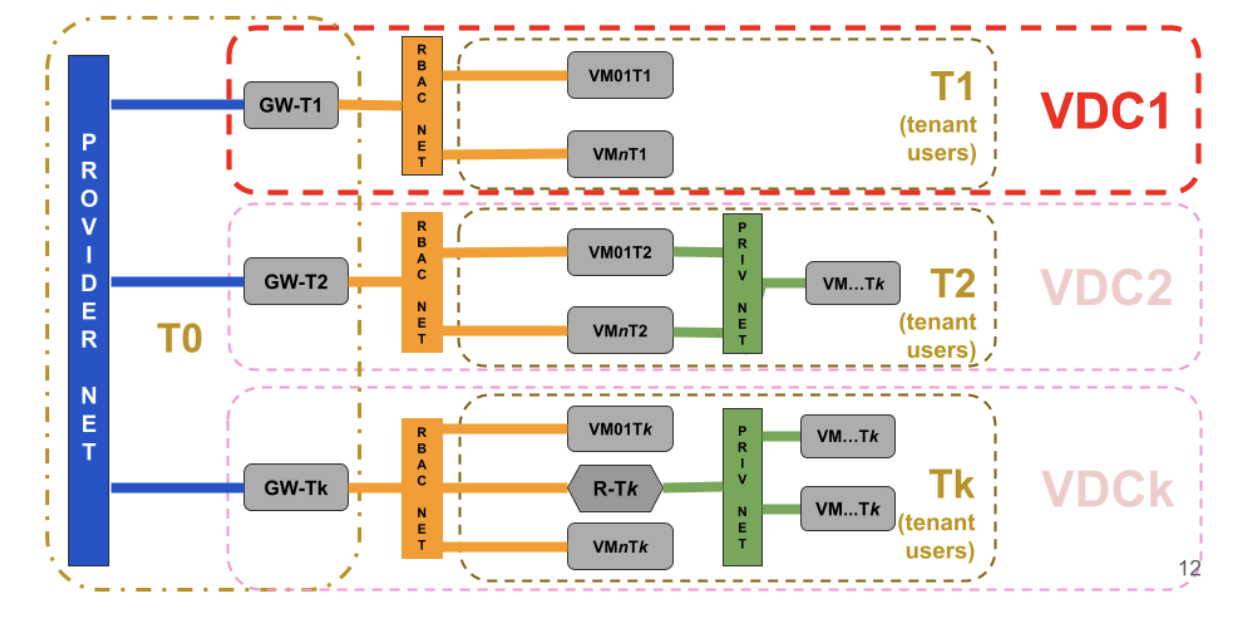
\includegraphics[width=0.6\textwidth]{figures/vdc-diagram.png}
    \caption{Schema di un Virtual Data Center}
    \label{fig:vdc}
\end{figure}
\section{Strumenti di Infrastructure-as-Code}
% introduzione in generale sull'infrastructure-as-code
\textit{Infrastructure-as-Code} (IaC) è una tecnologia con cui le istanze vengono configurate automaticamente al loro avvio installando pacchetti, scrivendo file di configurazione e inviando comandi alla shell.
Questo approccio porta diversi vantaggi allo sviluppo di infrastrutture\cite{cacciaguerra2024iac}:
\begin{itemize}
    \item{
        \textbf{Ripetibilità e coerenza}: l'utilizzo di un singolo script garantisce che ogni istanza sia configurata alla stessa maniera,
        riducendo il rischio di errori umani e garantendo coerenza.
    }
    \item{
        \textbf{Scalabilità}: l'automazione permette di scalare più rapidamente l'infrastruttura creando nuove istanze con la stessa configurazione.
    }
    \item{
        \textbf{Controllo versione}: gli script di configurazione possono essere versionati esattamente come il codice sorgente favorendo la tracciabilità delle modifiche e facilitando il rollback in caso di problemi.
    }
\end{itemize}
\subsubsection{Automazione e orchestrazione}
L'IaC permette di fare sia automazione che orchestrazione, ma questi sono due concetti diversi.\\
L'automazione cloud crea task ripetibili velocemente senza intervento umano come ad esempio la configurazione di una macchina,
mentre l'orchestrazione fornisce coordinazione tra più task automatizzate, gestendo, ad esempio, dipendenze ed ordine di esecuzione\cite{cacciaguerra2024iac}.

\subsection{Cloud-Init}
Durante l'implementazione del VDC sono stati valutati vari applicativi per l'automazione del deployment e l'orchestrazione:
\begin{itemize}
    \item \textbf{Heat}: il servizio integrato della suite OpenStack per orchestrare tramite template.
    \item {
        \textbf{Ansible}: un'altra valida alternativa a Cloud-Init che permette molta più libertà ed anche la possibilità di un mantenimento continuo delle istanze. 
        Necessita la configurazione di un nodo di controllo che gestisce la configurazione delle istanze tramite SSH tramite la scrittura di \textit{playbook}.
    }
    \item{
        \textbf{Cloud-Init}: un componente nativo di OpenStack che permette la configurazione automatica delle macchine virtuali al primo avvio tramite uno script. 
    }
\end{itemize}

I primi due sono soluzioni decisamente più complesse sia in termini di configurazione che di utilizzo da parte degli utenti, ma che offrono una maggiore flessiblità e potenza su larga scala.
Tuttavia Heat non era disponibile o non correttamente configurato. La sua assenza ha reso necessaria l'adozione di una soluzione alternativa già funzionante all'interno dell'infrastruttura.
Allo stesso tempo, Ansible, pur essendo un'ottima soluzione per la gestione di infrastrutture virtualizzate, richiede una configurazione iniziale più complessa e non è uno strumento adatto per chi si approccia
per la prima volta all'automazione.

Quindi la scelta è ricaduta su Cloud-Init per la sua semplicità d'uso: è sufficiente allegare uno script (user-data) al momento della creazione della macchina virtuale, e questa si configura automaticamente.
Un altro aspetto importante è che Cloud-Init opera una sola volta, al primo avvio della macchina scrive su file, configura l'istanza e installa pacchetti; non è pensato per un mantenimento a lungo termine che non è necessario,
anzi potenzialmente dannoso in questo contesto. 
Questo componente è già nativo di OpenStack e risulta il più semplice da utilizzare tra le alternative citate perché più agile nelle prime fasi di sviluppo e test in cui non si deve gestire deployment complessi, su larga scala o
di produzione bensì si ha bisogno di macchine virtuali pronte all'uso fin dal momento della loro creazione.
L'obbiettivo infatti, in un contesto di didattico e sperimentale come il VDC, è quello di semplificare al massimo l'esperienza di studenti e ricercatori, che non hanno competenze informatiche, senza introdurre strumenti che avrebbero richiesto una curva di apprendimento
rappresentando un ostacolo più che un valore aggiunto.

%
\section{Kubernetes}
\label{sec:kube}
%
% TODO: rileggere, andare a capo, typos, spiegazione componenti
%
Kubernetes è una piattaforma open-source per il deployment, la gestione e lo scaling automatico di applicazioni containerizzate. 
Operando direttamente a livello dei container fornisce diversi strumenti come autoscaling e bilanciamento del carico lasciando agli utenti la libertà di integrare componenti aggiuntivi per logging, monitoraggio e gestione personalizzata dell'infrastruttura.

Ciò apre ad una particolare flessibilità e possibilità di integrazione con ambienti cloud eterogenei. Non a caso, Kubernetes è fornito come servizio gestito (\textit{Platfrom-as-a-Service}) dai principali fornitori cloud tra cui: Azure Kubernetes Service (AKS), Google Kubernetes Engine (GKE), Oracle Kubernetes Engine (OKE).

Con l'avvento dei microservizi si è affermata come una delle principali piattaforme per l'implementazione di applicazioni scalabili, resilienti e portabili, diventando un elemento chiave nello sviluppo di applicazioni cloud-native.
\subsection{Principali componenti di Kubernetes}
Le applicazioni containerizzate sono dispiegate su entità chiamate Pods, questi ultimi sono assegnati ad uno o più nodi del cluster che possono essere macchine fisiche o virtuali.
In ogni nodo sono installati tutti i componenti necessari per controllare i pods mentre l'intero cluster è controllato dal nodo master (\textit{control plane}) che coordina il ciclo di vita dei pods, lo scheduling e la configurazione complessiva del cluster.
I principali componenti sono quindi:
\begin{itemize}
    \item {
        Nodi: macchine virtuali o fisiche dotate di tutti i componenti per la gestione dei containers. Ogni nodo contiene una container runtime (come CRI o \texttt{containerd}), \texttt{kubelet} (l'agente che gestisce localmente i Pods) ed opzionalmente \texttt{kube-proxy} che implementa una parte del networking.
    }
    \item {
        Pods: la più piccola unità di calcolo in Kubernetes. Ciascun pod contiene uno o più container, tipicamente uno solo oppure due se condividono le stesse risorse (es. pattern sidecar).
        I pod sono effimeri per natura, possono essere creati e distrutti dinamicamente.
    }
    \item {
        Services: un oggetto che astrae l'accesso ad un insieme di pod permettendo di esporli tramite un unico endpoint.
        Questo componente permette di gestire la natura effimera dei pod menzionata al punto precedente, evitando che l'utente debba conoscere l'indirizzo IP di ogni pod.
        Inoltre, fungono anche da Load Balancer interno per distribuire il traffico tra i vari pod.
    }
    \item {
        Ingress: è un servizio di rete che permette di smistare il traffico HTTP/HTTPS in base alle regole indicate dall'utente. Questo permette di erogare diversi servizi provenienti da diversi gruppi di pod dallo stesso endpoint.\\
        È un componente molto potente in quanto può fare da da terminatore SSL/TLS e Load Balancer, riducendo la necessità di configurarne uno esterno.
        È sempre necessario un Ingress Controller per applicare le regole di routing, questo può essere scelto dall'utente (come NginX o Traefik) o viene fornito dal cloud provider come nel caso di AKS, GKE o OKE. 
    }
    \item {
        Autoscaling: Kubernetes permette lo scaling orizzontale (aumentando il numero di Pods) o verticale (aumentando le risorse assegnate) al fine di mantenere entro una certa soglia l'utilizzo delle risorse,
        utilizzando componenti come Horizontal Pod Autoscaler (HPA) o strumenti di autoscaling esterni come Karpenter. 
        In ambienti cloud, Kubernetes è in grado di comunicare con il provider al fine di creare o rimuovere nodi dinamicamente ottimizzando costi e prestazioni.
    }
    \item {
        % TODO
        Storage: la gestione dello storage a lungo e corto termine. Viene fatto per mezzo di diversi componenti come volumi, volumi persistenti o ConfigMaps.
    }
\end{itemize}
\subsection{Container runtime e plugin CNI}
%
% TODO: rileggere, andare a capo, typos
%
Come menzionate in precedenza Kubernetes lascia all'utente la scelta di diversi componenti tra cui quello per gestire i container e quello per la gestione della rete\cite{kubernetes}.
Al fine di eseguire i container Kubernetes ha bisogno di un ambiente di esecuzione che implementi la \textit{Container Runtime Interface} (CRI).
Questa interfaccia permette di astrarre il layer di esecuzione dei container e permette a Kubernetes di essere indipendente dal tipo di container runtime utilizzato. 
Sarà quindi sufficiente che il container runtime implementi la CRI per essere utilizzato da Kubernetes, le più note implementazioni sono:
\begin{itemize}
    \item \textbf{Docker Engine}: utilizza internamente containerd e la sua installazione fornisce anche strumenti in linea di comando per la gestione dei container. 
        È necessario installare anche \texttt{cri-dockerd}, un adattatore che permette a Kubernetes e Docker di comunicare tramite la CRI.
    \item \textbf{containerd}: un gestore di container open-source appositamente sviluppato per il cloud che non necessita di nessun componente aggiuntivo. 
        Questo si interfaccia col sistema operativo per eseguire i container.
    \item \textbf{CRI-O}: un container runtime sviluppato per Kubernetes che implementa la CRI. Utilizza \texttt{runc} (come anche containerd) per eseguire i container ma potrebbe utilizzare
        tutti i runtime che implementano la Open Container Initiative (OCI).
\end{itemize}
Oltre al container runtime Kubernetes ha bisogno di un plugin che gestisca le comunicazioni all'interno del cluster; questo è
necessario per implementare il modello di rete di Kubernetes come l'assegnazione di indirizzi IP ai pod oppure l'implementazione dell'API Service.
Il plugin deve essere conforme con la \textit{Container Network Interface} (CNI) e ne sono disponibili varie distribuzioni, quella scelta per questo progetto è
\textit{Calico}.
%
\chapter{Implementazione}
% Introduzione al capitolo
In questo capitolo si affronterà l'implementazione effettiva del cluster a partire dal provisioning delle macchine che viene eseguito tramite interfaccia grafica
per poi passare alla configurazione delle macchine tramite Cloud-Init. Infine verrà affrontata la creazione del cluster, esponendo diverse alternative per il \textit{join}
di tutti i nodi.
\section{Provisioning delle macchine}
Le macchine virtuali vengono create tramite l'interfaccia grafica di OpenStack (Horizon). Viene scelto di allocare diverse risorse ai nodi, precisamente: 
\begin{itemize}
    \item Al nodo master vengono allocate più risorse rispetto ai nodi worker perché questo deve eseguire diversi processi per il mantenimento del cluster
        come \texttt{kube-proxy} per la gestione della rete, \texttt{kube-scheduler} per l'assegnazione dei pod ai nodi, \texttt{kube-apiserver} per la API di Kubernetes etc.
    \item Ai nodi worker viene allocata una quantità più moderata di risorse ma comunque sufficiente per eseguire diversi pods. 
\end{itemize}
Chiaramente queste risorse sono relative al carico di lavoro che il cluster deve affrontare, nel caso si attenda un lavoro più intenso o si stia progettando per un ambiente di produzione
si può decidere di avviare le macchine già con più risorse a disposizione.
\begin{figure}[!hbt]
    \centering
    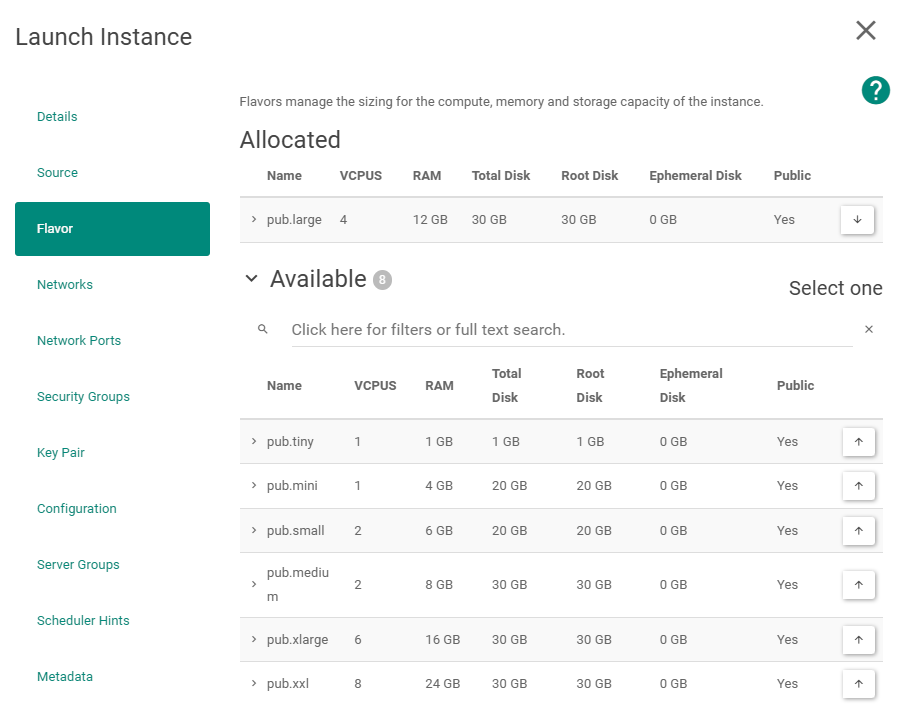
\includegraphics[width=0.8\textwidth]{figures/vm-nereide.png}
    \caption{Provisioning delle macchine virtuali su Nereide}
    \label{fig:kube-vm-provisioning}
\end{figure}
\FloatBarrier
Inoltre in ambienti di produzione è opportuno distribuire i componenti di controllo del cluster (\textit{control plane}) su più nodi master. In questo caso ciascun nodo master eseguirà un'istanza
di ciascun componente e le API verranno esposte al resto del cluster attraverso un load balancer che bilancerà il carico nei vari nodi master (v. \Cref{fig:kube-ha-topo}). È indicato distribuire i nodi in diversi datacenter 
(chiamati negli ambienti cloud \textit{availability zones}) per mitigare il rischio di interruzione dei servizi\cite{kubernetes}.
%
\begin{figure}[!hbt]
    \centering
    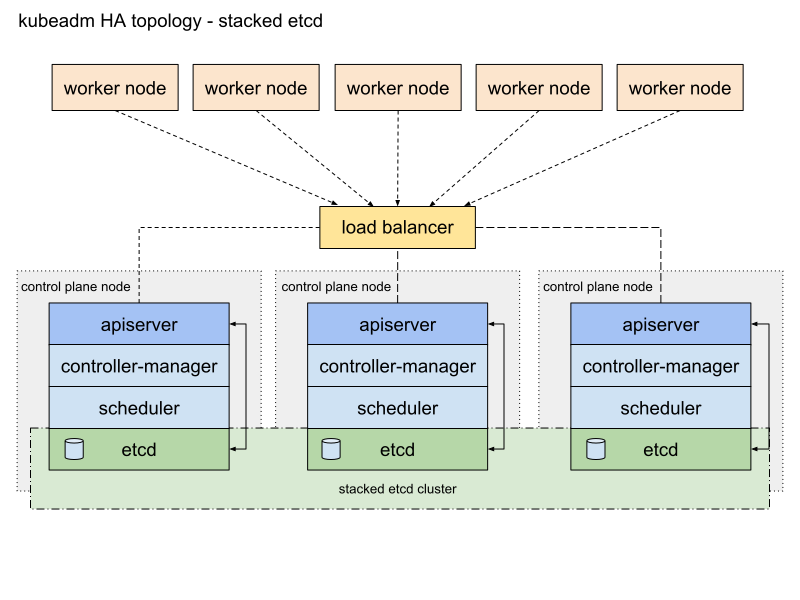
\includegraphics[width=0.8\textwidth]{figures/kube-ha-topo.png}
    \caption{Possibile architettura di un cluster Kubernetes ad alta disponibilità}
    \label{fig:kube-ha-topo}
\end{figure}
%\
\FloatBarrier
\section{Configurazione ed installazione dei pacchetti}
Cloud-Init si occupa dell'installazione e configurazione preliminare dei nodi, in particolare:
\begin{itemize}
    \item aggiunge le repository poi installa i pacchetti necessari per il funzionamento del cluster: \texttt{containerd}, \texttt{kubeadm}, \texttt{kubectl} e \texttt{kubelet}
    \item {l'impostazione di \texttt{Systemd} come cgroup manager per \texttt{containerd} e Kubernetes.
        \lstinputlisting[language=bash,label={lst:systemd-cgroup}, firstline=37, lastline=37]{listings/master.yaml}
    }
    \item {
        l'attivazione di \textit{ip forwading} per permettere ai nodi di scambiare pacchetti tra di loro.
        \lstinputlisting[language=bash,label={lst:systemd-cgroup}, firstline=40, lastline=40]{listings/master.yaml}
    }
    \item l'installazione del plugin CNI \textit{Calico} per la gestione della rete
    \item {
        infine, l'avvio del cluster
        \lstinputlisting[language=bash,label={lst:systemd-cgroup}, firstline=54, lastline=54]{listings/master.yaml}
    }
\end{itemize}
Un cluster composto da un nodo master e tre nodi worker sarà composto come in \Cref{fig:kube-cluster}. Tutti i nodi sono inseriti nella rete interna del VDC ed un gateway permette l'accesso
dall'esterno del cluster sia per il controllo delle macchine sia per l'accesso ai servizi.\\
Ovviamente l'architettura del cluster cambia in base all'ambiente in cui viene disposto.
\begin{figure}[!hbt]
    \centering
    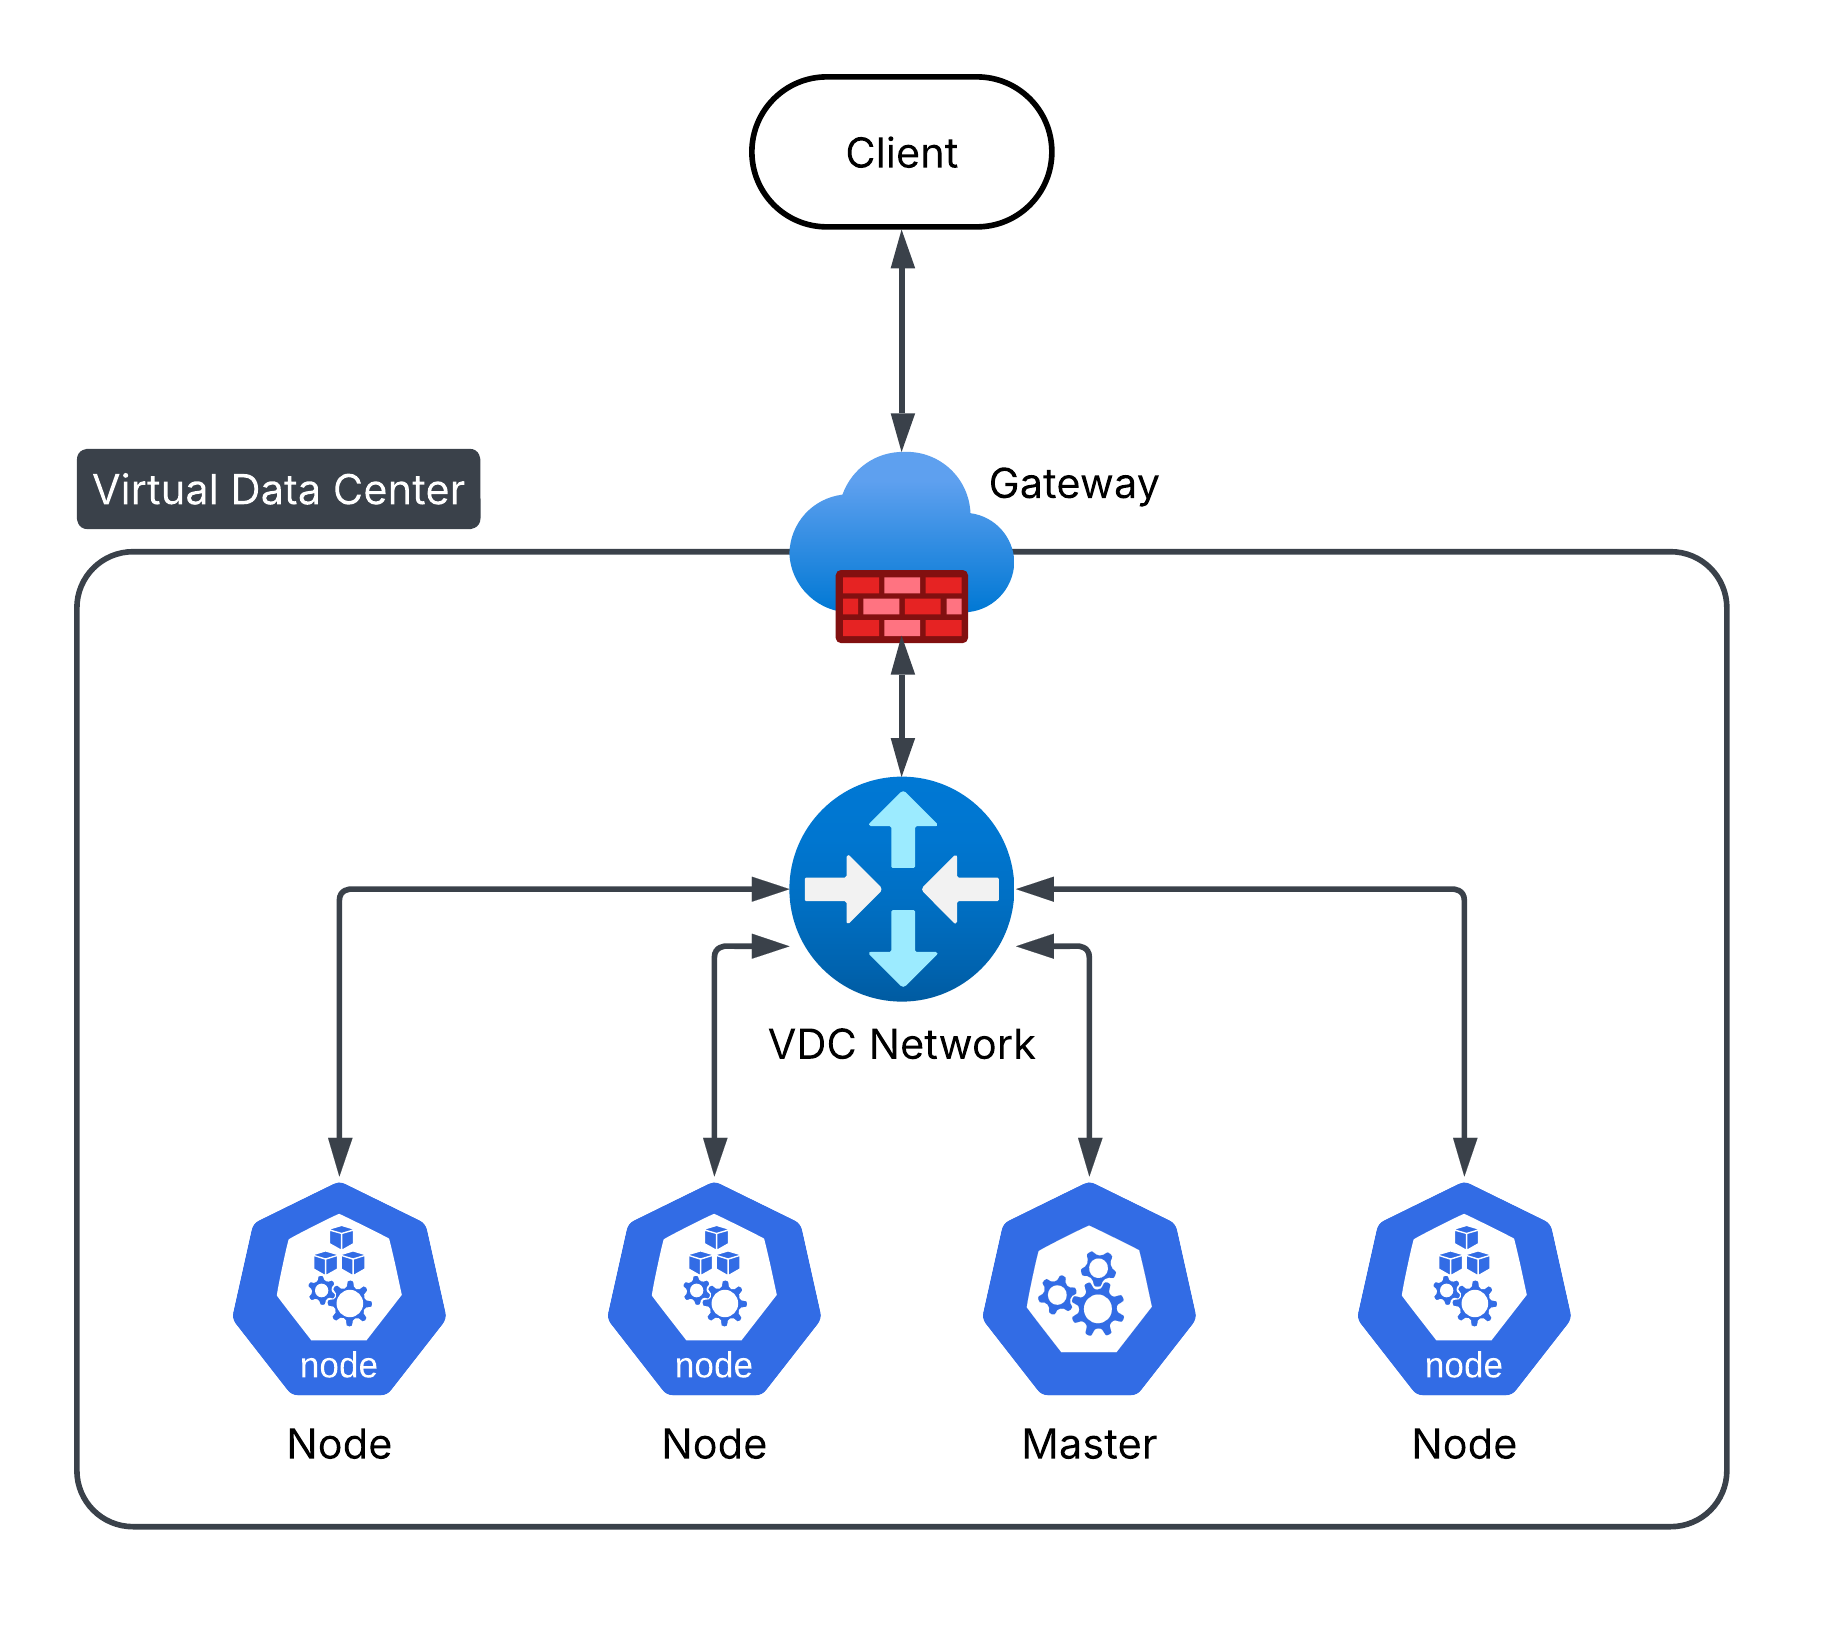
\includegraphics[width=0.5\textwidth]{figures/kube-vdc.png}
    \caption{Schema del cluster disposto su un VDC}
    \label{fig:kube-cluster}
\end{figure}
\section{Creazione del cluster}
\label{sec:cluster-creation}
Dopo aver installato i pacchetti necessari e configurato i nodi, processo che può richiedere diversi minuti, si può procedere alla creazione del cluster vero e proprio,
ciò consiste nell'integrazione dei nodi worker nel cluster. Questa operazione non è completamente automatizzabile in quanto utilizzando
l'interfaccia grafica in congiunzione con \texttt{kubeadm} è necessario reperire un token di autenticazione che poi va inserito nei nodi worker.\\
Questo token viene generato dal nodo master e non è conosciuto a priori.\\
A questo punto si può procedere in diversi modi:
\begin{itemize}
    \item Lasciare questo processo in manuale, l'utente dovrà accedere al master, copiare il comando e poi eseguirlo in ciascun nodo worker
    \item Implementazione di script che gestiscano automaticamente l'integrazione dei nodi worker, essenzialmente automatizando ciò che fa l'utente nel punto precedente
\end{itemize}
Nel primo caso sarà sufficiente generare il comando manualmente sul nodo master per poi accedere in SSH a ciascun nodo worker ed eseguire il comando.\\
Nel secondo caso viene implementato uno script bash che esegue l'operazione in automatico sul nodo master e poi lo esegue, connettendosi in SSH, in ciascun nodo worker. 
Questo script deve essere eseguito mentre si è connessi alla rete VPN che permette l'accesso al VDC dal proprio terminale, in più bisogna scrivere su un file di testo l'indirizzo IP del nodo master e dei nodi worker.
Successivamente lo script si occuperà di leggere il file e di eseguire i comandi necessari per l'integrazione dei nodi worker (v. \Cref{lst:join-script}).
\lstinputlisting[float, language=bash, label={lst:join-script}, caption=Script di integrazione dei nodi worker]{listings/join-nodes.sh}

L'alternativa più completa ed automatizzata per la creazione del cluster può essere quella di utilizzare l'interfaccia in linea di comando di OpenStack.
Tramite questa si ha un controllo più granulare sulle operazioni, infatti l'interfaccia grafica di OpenStack non offre tutte le funzionalità disponibili tramite linea di comando.
Integrando questo strumento con script bash opportunamente costruiti si può automatizzare completamente il processo.
Questo aspetto viene affrontato anche negli sviluppi futuri del progetto alla \Cref{sec:future}.
\subsection{Configurazione di un controller Ingress}
\label{sec:ingress}
Infine viene installato l'Ingress Controller, per questa implementazione è stato scelto \textit{NginX Ingress Controller}. Questo componente è solitamente
incluso nel servizio di Kubernetes dei cloud provider ma in questo caso è necessario comportarsi come se si stesse lavorando su macchine fisiche usando la 
versione \textbf{bare-metal} del controller.\\
Infatti nelle implementazioni su cloud, il controller funge anche da Load Balancer per l'accesso al cluster ed esso collabora con il servizio che espone il cluster all'esterno
mentre nel VDC è il gateway a gestire l'accesso ed il resto dell'infrastruttura a gestire il bilanciamento del carico. Questa configurazione costringe il controller ad assumere 
un ruolo diverso, ovvero quello di gestire il traffico all'interno del cluster.
Qui si possono scegliere due modalità di configurazione, anche in funzione delle operazioni che si vorranno svolgere nel cluster\cite{nginx-ingress-controller}:
\begin{itemize}
    \item \textbf{Utilizzo di MetalLB}: una soluzione unicamente software che permette l'utilizzo di load balancer anche in ambienti che non ne implementano.
        È comunque necessario che il cluster possa essere esposto all'esterno tramite un indirizzo IP pubblico. MetalLB si occupa di assegnare ad ogni servizio un
        indirizzo IP ed utilizza un nodo come punto di ingresso per il traffico esterno, successivamente annuncia tramite ARP che un servizio è raggiungibile tramite 
        quel nodo.\\
        Questo metodo non è implementabile perché il cluster è protetto da firewall mentre MetalLB ha bisogno di essere esposto completamente alla rete.
    \item {\textbf{Esposizione tramite NodePort}: un metodo decisamente più semplice che consiste in impostare l'Ingress Controller in modalità NodePort.
        In questo modo il traffico esterno viene inviato ad una porta specifica di uno qualsiasi dei nodi del cluster, che poi lo inoltra al controller (che poi
        eseguirà il routing verso i servizi).\\
        In questo progetto è stata scelta questa modalità sia per motivi di semplicità nel testing sia perché il contesto non permette l'utilizzo di MetalLB.
    }
\end{itemize}
\chapter{Testing}
\section{Deployment di prova}
\subsection{Architettura di test}
\label{sec:test-depl}
Per verificare il corretto funzionamento del cluster viene eseguita una semplice applicazione web stateless utilizzando NginX come server web. Il deployment consiste in due applicazioni
posizionate su più pod che servono due pagine web distinte, come per simulare l'erogazione di due servizi diversi.

I pod vengono racchiusi in un servizio che espone il suo endpoint al cluster; infine una risorsa Ingress espone il servizio all'esterno del cluster,
con le modalità menzionate alla \Cref{sec:ingress}, instradando il traffico verso i servizi in base al percorso richiesto.
\begin{figure}[!hbt]
    \centering
    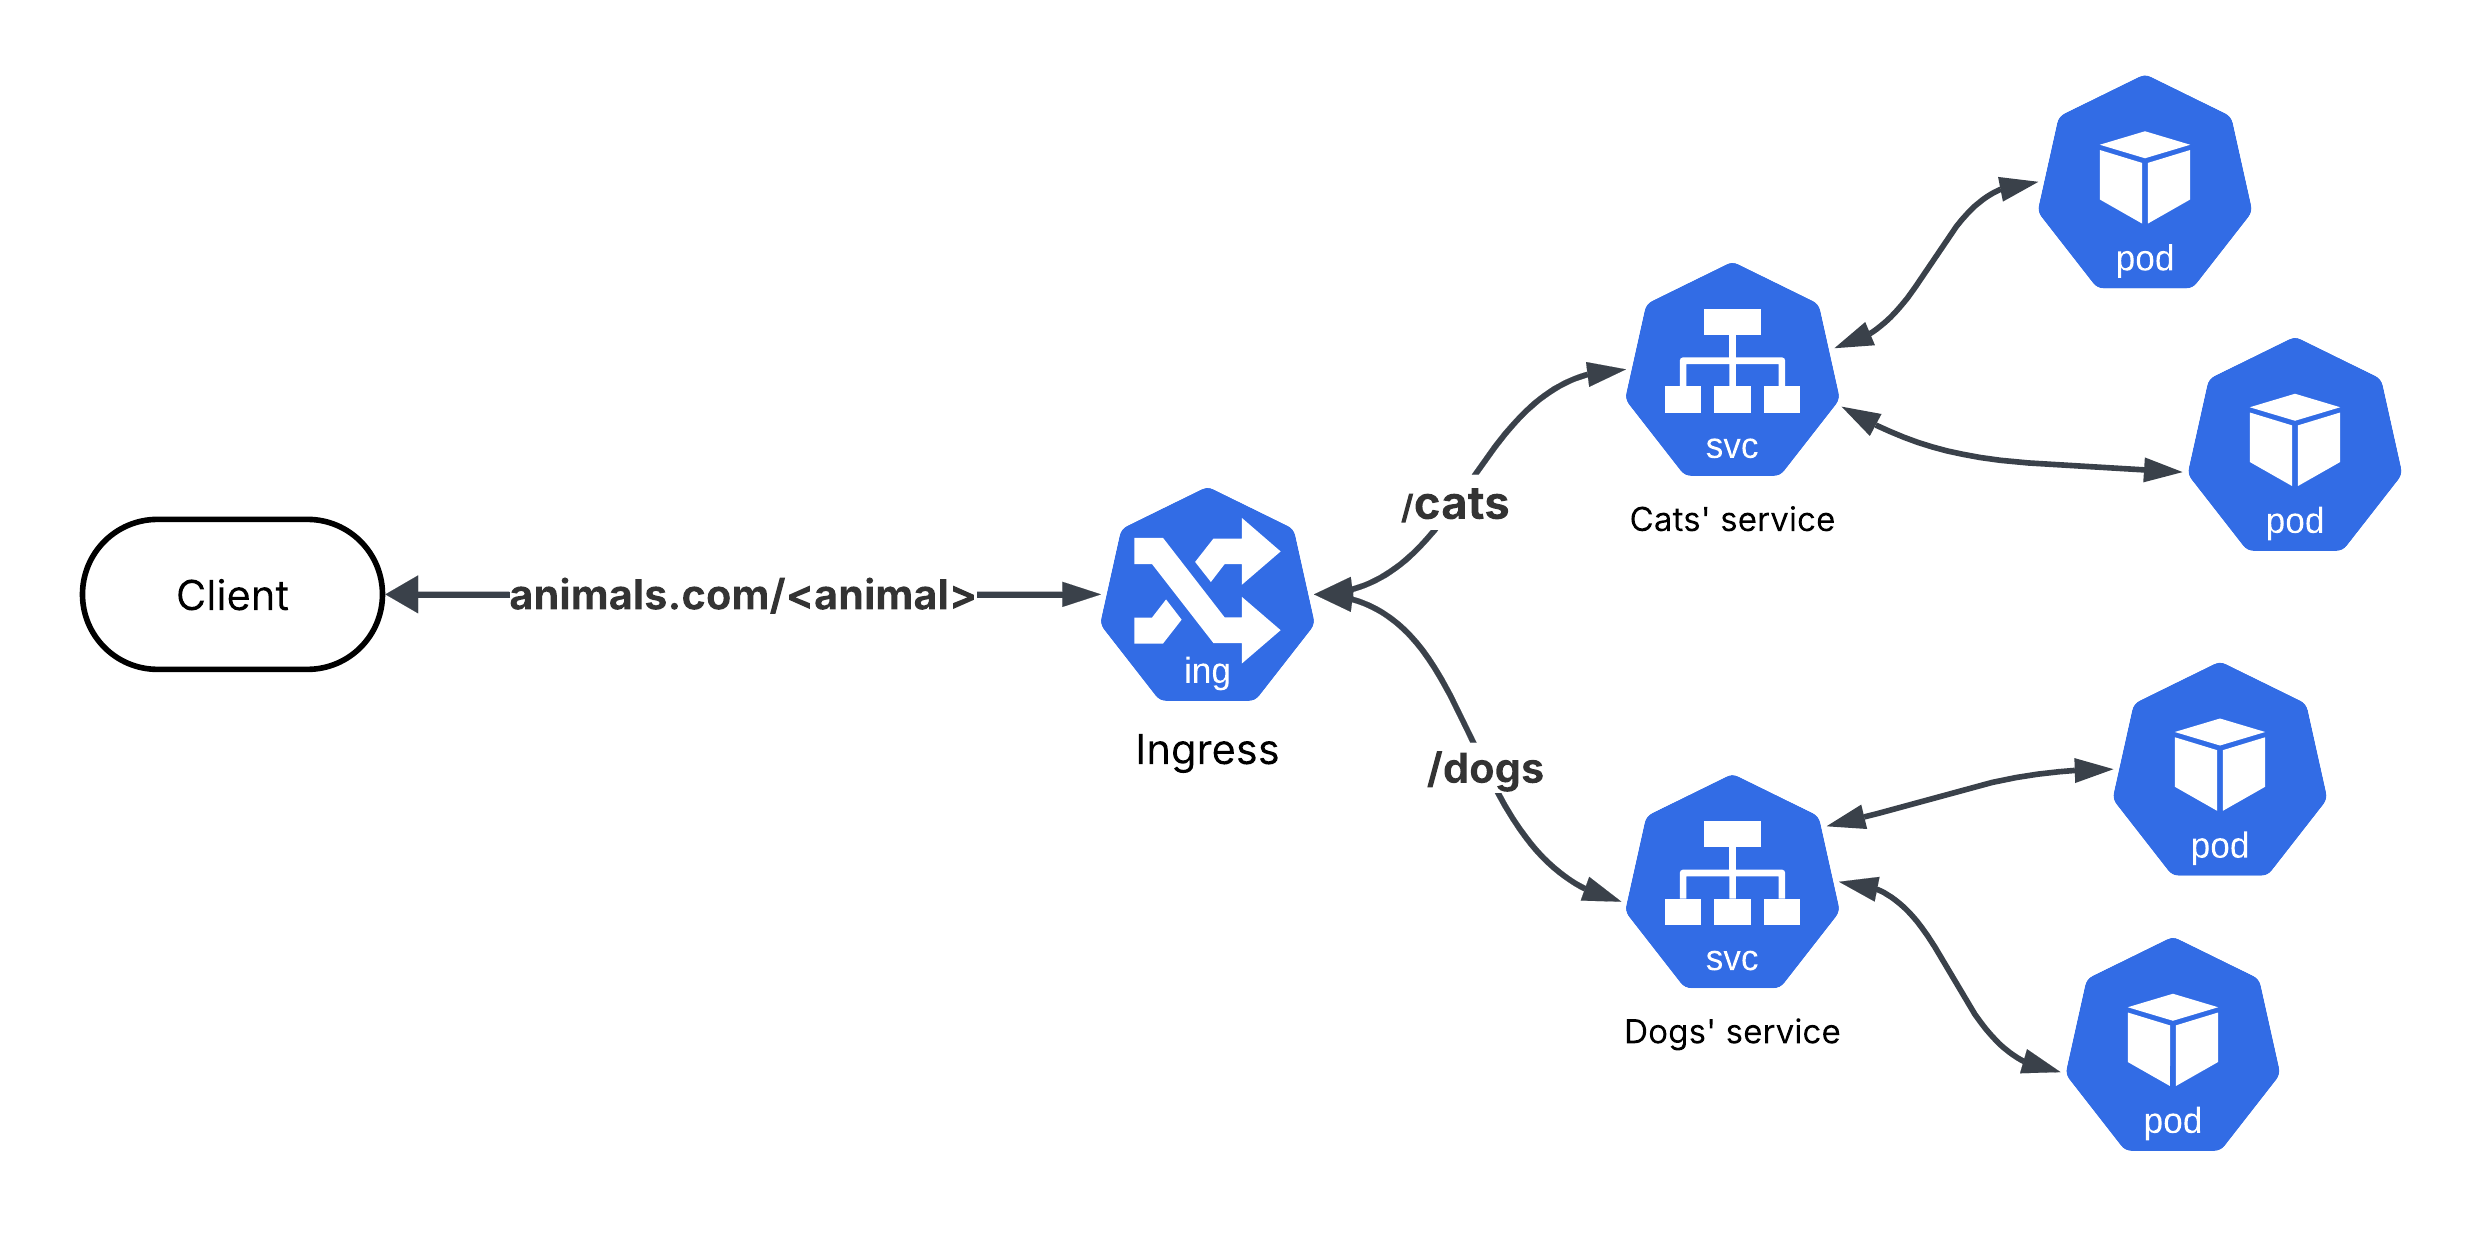
\includegraphics[width=0.9\textwidth]{figures/test-deployment.png}
    \caption{Schema logico del deployment di prova}
    \label{fig:test-deployment}
\end{figure}
\FloatBarrier
\subsection{Architettura all'interno del VDC}
Dal punto di vista del VDC, l'aspetto del cluster sarà come in \Cref{fig:test-vdc}. Le richieste HTTP possono essere inoltrate al cluster tramite uno qualsiasi dei nodi,
coerentemente alla modalità di esposizione scelta per l'Ingress Controller, alla porta scelta per il NodePort. Si potrà quindi scegliere un qualsiasi nodo del cluster 
da esporre tramite il firewall del VDC.
\begin{figure}[!hbt]
    \centering
    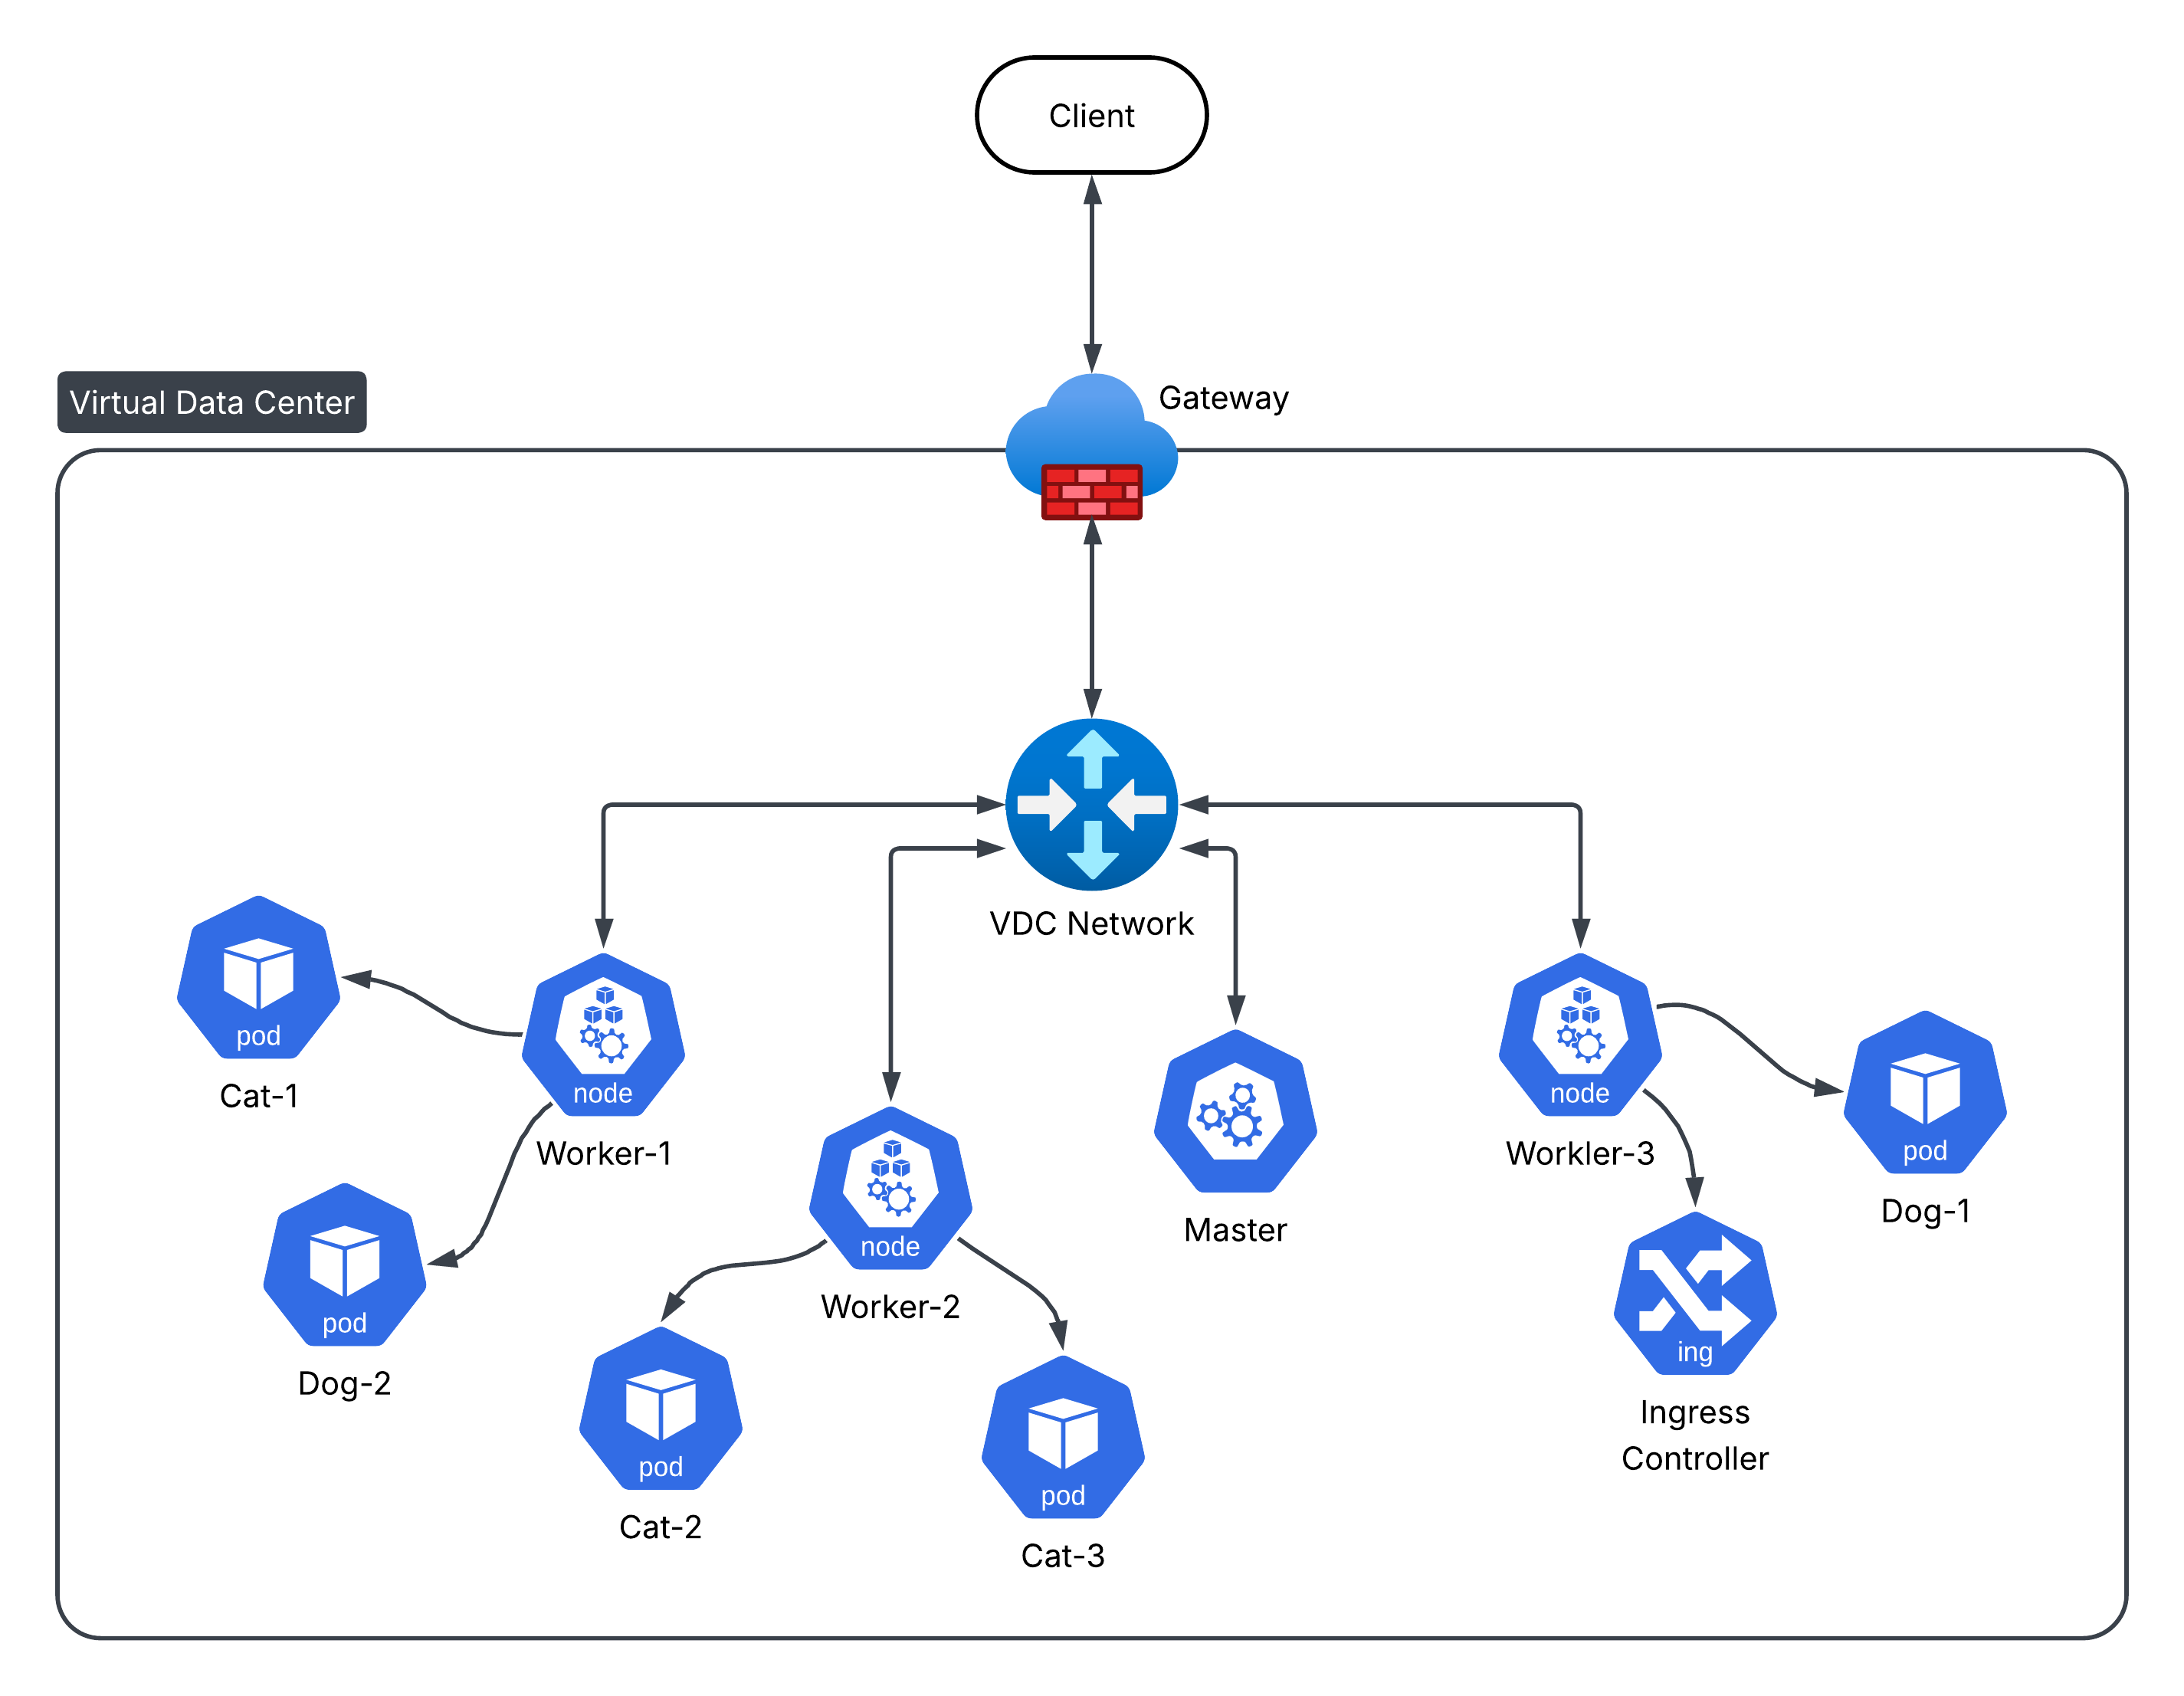
\includegraphics[width=0.9\textwidth]{figures/test-vdc.png}
    \caption{Schema del cluster all'interno del VDC (la distribuzione dei pod sui nodi è un esempio)}
    \label{fig:test-vdc}
\end{figure}
\FloatBarrier
\subsection{Esecuzione del test}
Il deployment viene applicato tramite i seguenti comandi:
\begin{lstlisting}
$ git clone https://github.com/bagarozzi/minikube-examples.git examples
$ kubectl apply -R -f examples/minikube/multiple-ingress/manifests
\end{lstlisting}
Prima di verificare il funzionamento bisogna recuperare la porta su cui è esposto, su ciascun nodo, l'Ingress Controller:
\begin{lstlisting}
$ kubectl get svc -n ingress-nginx                
\end{lstlisting}
Troveremo il numero di porta alla colonna \texttt{PORT(S)} della riga corrispondente al servizio \texttt{ingress-nginx-controller}.
Ora è possibile verificare il funzionamento in locale tramite \texttt{curl}. Il risultato sarà quello indicato al \Cref{lst:output-local}.
\begin{lstlisting}
$ curl -i -H "Host: www.animals.com" http://127.0.0.1:30900/cats
\end{lstlisting}
Successivamente si espone il cluster all'esterno aggiungendo una regola di port forwarding al firewall del VDC. Tramite questa si va a ridirezionare il traffico in ingresso verso
un nodo qualsiasi del cluster (master incluso), sulla porta NodePort dell'Ingress Controller.
\begin{figure}[!hbt]
    \centering
    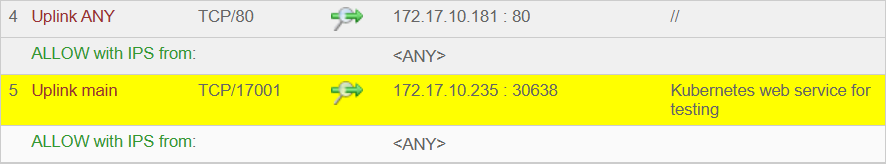
\includegraphics[width=0.8\textwidth]{figures/forwarding-rule.png}
    \caption{Regola di port forwarding nel firewall del VDC}
    \label{fig:firewall-rule}
\end{figure}
Infine si verifica la disponibilità del servizio da un'altra macchina non collegata alla rete interna del VDC. 
\begin{lstlisting}
$ curl -i -H "Host: www.animals.com" http://gw-ingv-labdidattica.pp.ingv.it:17001/cats
\end{lstlisting}
Visto che il dominio utilizzato (\texttt{www.animals.com}) non è inserito in nessun DNS non sarà possibile scrivere direttamente l'URL ma si dovrà aggiungere manualmente
l'indirizzo all'header della richiesta. In questo modo quando la richiesta viene inoltrata attraverso da Ingress questo saprà quale host si sta richiedendo,
senza questo accorgimento la richiesta arriverebbe al controller ma non verrebbe inoltrata a nessun servizio perché il campo header conterrebbe un altro dominio. 
\lstinputlisting[float, language=bash,label={lst:output-local}, caption=Output della richiesta cUrl]{listings/test-output.txt}
\section{Considerazioni sui test}
\label{sec:test-concl}
Se eseguiti con successo, i test della \Cref{sec:test-depl} dimostrano una piena funzionalità del cluster nello svolgere le operazioni di base come creazione di pods, servizi e routing di Ingress.
Tuttavia è importante osservare come questi non siano completamente esaustivi e siano un primo passo per dimostrare la fattibilità ed il funzionamento del sistema; sarà cura dei futuri utilizzatori e sviluppatori di questo progetto mantenere i componenti aggiornati e compatibili tra
di loro nel caso vengano utilizzati add-ons, plugin o funzionalità aggiuntive.
Inoltre, i test non coprono aspetti di performance del cluster, che sono fondamentali in un ambiente di produzione. Per esempio, sarà opportuno 
aumentare il numero di risorse allocate ai nodi ed il numero di nodi stessi nel caso si vogliano implementare servizi onerosi. 
Per quanto riguarda la sicurezza, questa è garantita dal VDC stesso che implementa un firewall e regole che limitano l'accesso alle macchine virtuali dall'esterno.
%
\chapter{Conclusione e lavori futuri}
Lo scopo di questo progetto era quello di verificare la fattibilità dell'automazione di un cluster Kubernetes su un VDC. 
E' stato dimostrato il provisioning e la configurazione automatica delle macchine virtuali tramite script bash e Cloud-Init, che in pochi minuti permettono di 
avere un cluster Kubernetes funzionante e pronto per l'uso.\\
Questo permette ancora una volta di portare avanti quello che è il principio su cui sono stati creati i VDC: permettere ai suoi utenti un'infrastruttura dinamica
su cui basare le proprie ricerche e sviluppi.
E' stato anche disposto un semplice test di funzionamento del cluster, che ha dimostrato la possibilità di eseguire applicazioni containerizzate e di esporle all'esterno.

Sarà compito dei futuri sviluppatori e Data Scientists implementare i servizi che desiderano erogare dalla piattaforma, rendendo questo progetto più completo.
Le conseguenze sono, per l'appunto, che il cluster non è adatto per un utilizzo di produzione e che non sono stati implementati test di sicurezza, resilienza o performance
come menzionato nella \Cref{sec:test-concl}.
D'altra parte lo scopo del progetto ed il contesto in cui si inserisce non necessita di ulteriore sviluppo e sarà oggetto di futuri lavori l'espansione del progetto.
\section{Sviluppi futuri}
\label{sec:future}
Al fine di rendere il progetto più completo e pronto per un utilizzo in produzione si possono fare i seguenti sviluppi:
\begin{itemize}
    \item {\textbf{Monitoraggio}: implementazione di un sistema di monitoraggio e logging (come Grafana e Prometheus) per tenere traccia dello stato del cluster, dei servizi e degli oggetti.
    Questo permetterebbe di individuare problemi e risolverli in modo più rapido oltre che a tracciare l'utilizzo delle risorse e l'efficienza dei servizi.
    }
    \item{
        \textbf{Resilienza}: introduzione di molteplici copie del nodo master per aumentare la resilienza del cluster. Questo comporterà l'introduzione di un load balancer per dividere il traffico tra i nodi master.
        In più si possono introdurre più istanze di \texttt{etcd} (il database che contiene lo stato del cluster)\cite{kubernetes}.
    }
    \item {
        \textbf{Ordinaria amministrazione}: assicurarsi che il cluster rimanga sicuro aggiornando i componenti e rinnovando i certificati (se deve rimanere
        attivo per un lungo periodo di tempo), che i nodi rimangano aggiornati e con il corretto numero di risorse allocate ed introdurre un numero di efficientamenti
        per migliorare la salute del cluster; le buone prassi per la gestione di un cluster sono introdotte nella documentazione ufficiale e dipendono dall'utilizzo che
        si vuole fare del cluster stesso\cite{kubernetes}.
    }
\end{itemize}
Come menzionato alla \Cref{sec:cluster-creation}, un altro aspetto che può essere migliorato è l'automazione della creazione del cluster.
Per ottenere il massimo livello automazione sarebbe preferibile disporre dello strumento in riga di comando di OpenStack, che se integrato con script bash, renderebbe 
più veloce sia il provisioning (sarebbe sufficiente un comando unico per creare tutte le macchine) sia l'integrazione dei nodi nel cluster tramite il recupero del token di accesso.
%Fornire l'accesso all'interfaccia in riga di comando a tutti gli utenti del VDC 

%----------------------------------------------------------------------------------------
% BIBLIOGRAPHY
%----------------------------------------------------------------------------------------

\backmatter

\nocite{*} % Include all bibliography entries, even uncited ones

\bibliographystyle{ieeetr}
\bibliography{bibliography}

\begin{acknowledgements} % this is optional
Optional. Max 1 page.
\end{acknowledgements}

\end{document}
